\documentclass[a4paper, 11pt, notitlepage]{article}
\addtolength{\hoffset}{-1cm}
\addtolength{\textwidth}{2cm}
\usepackage[utf8]{inputenc}
\usepackage[frenchb]{babel}
\usepackage[T1]{fontenc}

\usepackage{multicol}
\usepackage{listings}
\usepackage{pdfpages}
\usepackage{hyperref}

\usepackage{color}
\definecolor{lightgray}{rgb}{.9,.9,.9}
\definecolor{darkgray}{rgb}{.5,.2,.2}
\definecolor{purple}{rgb}{0.65, 0.12, 0.82}
\definecolor{brown}{RGB}{140, 0, 0}


\lstnewenvironment{java}
                  {\lstset{
                      language=Java,
                      breaklines=true,
                      showstringspaces=false,
                      commentstyle=\color{red},
                      stringstyle=\color{darkgray},
                      identifierstyle=\ttfamily,
                      keywordstyle=\color{blue},
                      basicstyle=\footnotesize,
                     escapeinside={(*}{*)},
                      frame=single,
                      numbers=left,
                      %xleftmargin=0.08\textwidth
                    }
                  }
                  {}


%%%%%%%%%%%%%%%%%%%%%%%%%%%%%%%%%%%%%%%%%%%%%%%%%%%%%%%%%%%%%%%%%%%%%%%%%%%%%%

\title{
  \huge Rapport de projet \\
  \huge CPS : River City Ransom\\
}
\author{
  Béatrice CARR\'E \\
  Steven VAROUMAS \\
  \\
}

\begin{document}
\maketitle
\section*{Introduction}


Le projet de cette année pour l'UE CPS  consistait à développer un jeu : \emph{River City Ransom}
TODO explication projet

Pour cela, nous avons suivi la méthodologie apprise en cours blablablablbala

La méthodologie pour la \emph{conception par contrat}  se compose de trois phases :
\begin{enumerate}
\item Analyse : spécifications algébriques 
\item Conception : par contrat à partir des spécifications
\item Implémentation : garantie vis-à-vis des contrats
\end{enumerate}
Nous avons suivi scrupuleusement chacune de ces étapes pour l'élaboration du
projet et ainsi honorer notre contrat défini. 
Dans ce rapport, seront présentées la méthodologie utilisée pour
réaliser ce projet, ainsi que les difficultés rencontrées.
 
Ensuite, notre réalisation du procédé appliqué
et les solutions apportées au problème posé vous seront détaillées.





%%%%%%%%%%%%%%%%%%%%%%%%%%%%   Problème   %%%%%%%%%%%%%%%%%%%%%%%%%%%%


\section{Problème posé}

INTRO = problème posé non ?? 
Le problème est de rester cohérents tout au long des phases d'analyse,
de conception et d'implémentation, tout en respectant la méthodologie de la \emph{conception par contrat},
pour ainsi obtenir un programme tout aussi cohérent et fiable.

\subsection{Analyse : la specification}
Le but de la spécification est de reconnaître les éléments logiques
d’un programme à partir d’une définition du jeu River City Ransom.
Pour chaque service décrit, il faut en sortir une spécification la
plus détaillée et complète possible.

Une grande partie des opérateurs d'un service requièrent la validité de plusieurs pré-conditions permettant leur appel. De la même façon, plusieurs post-conditions définissent quelle est l'action de l'opérateur sur le service en question.

Nous avons rencontré plusieurs difficultés :
\begin{itemize}
\item Les problèmes d’interprétation personnelle, qui peuvent être
  très différentes selon les membres du groupe de travail.
\item Le manque d'information dans la description de chaque service
  est à compléter avec son imagination, qui doit être réaliste.
\item Il faut rester cohérents au fur et à mesure de la création de
  chaque service, pour avoir le moins possible à revenir aux services
  déjà traités. 
\item Il est important de garder en tête la notion de référentiel pour
  chaque service, qui permet de ne pas traiter des éléments qui
  le concerneraient de l'extérieur, et donc de ne pas définir dans celui-ci.

\item La représentation de certains éléments nous a parue difficile,
  comme pour une liste ou encore la notion de temps.
\end{itemize}

\subsection{Tests}
La seconde phase est de décrire et d'implémenter les tests pour préparer
le respect du contrat lors de la dernière phase.

Celle-ci est importante dans la mesure où elle représente le liens
entre la spécification et l'implémentation pure, tant au niveau des
conditions, qu'au niveau de TODO.

Pour n conditions sur chaque opération $\Rightarrow$ (2 à $\sim 6)^n$ tests!
Pour chaque argument de méthode, il faut trouver les valeurs à tester.
Si booléen, il suffit de tester avec true et false.
Mais si entier float string etc, il est impossible de tester toutes
les valeurs. Il faut donc sélectionner les valeurs les plus
pertinentes à tester, qui sont en général les valeurs juste avant et
après les limites d'intervales de tests ainsi qu'une valeur centrale. \\


Par exemple, l'observateur \emph{bloc(T,x,y)} du service \emph{Terrain} possède ce qui semble être deux préconditions simples :  0 $\le$ x $\le$ largeur(T) et 0 $\le$ y $\le$ profondeur(T) \\


Ce qui se traduit en réalité par 4 conditions :
\begin{itemize}
\item 0 $\le$ x 
\item x $\le$ largeur(T)
\item 0 $\le$ y
\item y $\le$ profondeur(T) \\
 
 \end{itemize} 
 

 Pour avoir une étendue de test satisfaisante, il nous faudrait \underline{au moins} tester pour chaque condition une situation qui rendrait la condition fausse et une situation qui rendrait la condition vraie. \\
 
 On peut alors écrire une table de vérité afin d'avoir une idée des différents tests à réaliser, selon les cas :
 
 \begin{center}
   \begin{tabular}{ | c | c | c | c |}
     \hline
     0 $\le$ x &  x $\le$ largeur(T) & 0 $\le$ y &  y $\le$ profondeur(T) \\ \hline
    $\top$ & $\top$ & $\top$ & $\top$ \\ \hline
    $\top$ & $\top$ & $\top$ & $\bot$ \\ \hline
    $\top$ & $\top$ & $\bot$ & $\top$ \\ \hline
    $\top$ & $\top$ & $\bot$ & $\bot$ \\ \hline
    $\top$ & $\bot$ & $\top$ & $\top$ \\ \hline
    $\top$ & $\bot$ & $\top$ & $\bot$ \\ \hline
    $\top$ & $\bot$ & $\bot$ & $\top$ \\ \hline
    $\top$ & $\bot$ & $\bot$ & $\bot$ \\ \hline
    
    $\bot$ & $\top$ & $\top$ & $\top$ \\ \hline
    $\bot$ & $\top$ & $\top$ & $\bot$ \\ \hline
    $\bot$ & $\top$ & $\bot$ & $\top$ \\ \hline
    $\bot$ & $\top$ & $\bot$ & $\bot$ \\ \hline
    $\bot$ & $\bot$ & $\top$ & $\top$ \\ \hline
    $\bot$ & $\bot$ & $\top$ & $\bot$ \\ \hline
    $\bot$ & $\bot$ & $\bot$ & $\top$ \\ \hline
    $\bot$ & $\bot$ & $\bot$ & $\bot$ \\ \hline

   \end{tabular}
 \end{center}

Soient 16($=2^4$) tests à réaliser.  \\

Certains opérateurs (ou constructeurs) possèdent jusqu'à 8 préconditions, ce qui reviendrait à effectuer au moins $2^8=256$ tests. \\


Théorie : tous les tests réussissent signifierait que nous avons une application sans erreurs À VÉRIFIER

Réalité : il faut aussi que l’implémentation respecte ce qui est
demandé, et toutes les valeurs ne sont pas testées, il est donc
impossible d'être sûrs. A DÉVELOPPER 


\subsection{Implémentation par contrat}
développer les services et conditions soulevés, en respectant le
squelette étudié.






%%%%%%%%%%%%%%%%%%%%%%%%%%%%   Solution   %%%%%%%%%%%%%%%%%%%%%%%%%%%


\section{Solution}
petite intro ?

\subsection{Specification}

La spécification que nous avons réalisé contient les services suivants : 

\begin{itemize}
\item \textbf{Personnage} qui décrit les comportements des personnages du jeu (Ryan et Alex).
\item \textbf{Gangster} qui raffine les comportements des personnages pour les ennemis de Ryan et Alex.
\item \textbf{Bloc}, qui représente un bloc situé sur sol du terrain de jeu.
\item \textbf{Objet}, définissant les caractéristiques des objets éparpillés sur le sol et pouvant être ramassés par les personnages.
\item \textbf{Terrain}, représentant le terrain (en trois dimensions) dans lequel les personnages évoluent.
\item \textbf{MoteurJeu}, service gérant les tours de jeu ainsi que vérifiant l'état de la partie.
\item \textbf{GestionCombat} qui est le service central de l'application, et qui s'occupe en particulier d'associer à chaque commande envoyée à un personnage des actions concrètes dans le jeu. \\
\end{itemize}

Ces services décrivent de nombreux comportements, tous précisés en annexe. Nous nous attacherons ici à préciser quels ont été nos décisions particulières lors de la conception de leur spécification: \\

\begin{itemize}

\item Dans le service \emph{Personnage}, nous avons choisi de séparer l'action de ramasser (un objet ou un personnage) en trois opérateurs différents : ramasser\_objet, ramasser\_argent, et ramasser\_perso. L'idée était ici de permettre à un personnage de ramasser de l'argent sans pour autant se retrouver dans l'impossibilité de ramasser un autre objet par la suite ou bien de continuer à ramasser de l'argent alors qu'il est équipé d'une arme (ou d'un personnage) \\

\item Le service \emph{Gangster} n'est qu'un raffinement du service \emph{Personnage} sur lequel les opérateurs concernant l'argent (\emph{ramasser\_argent}, \emph{depot\_argent}, etc.) n'ont pas d'influence.  \\

\item Chaque \emph{Bloc} possède un observateur \emph{type} qui retourne si le bloc est \emph{VIDE} (il ne contient aucun objet ou trésor), \emph{FOSSE} (il représente un trou dans lequel les personnages peuvent tomber) ou \emph{OBJET} (il contient un objet, qui peut être un trésor ou une arme).  \\

\item Nous avons décidé qu'il ne pourrait y avoir qu'un seul objet (au maximum) par bloc sur le sol du terrain de jeu. Ainsi, il est impossible pour un personnage de jeter un objet s'il ne se situe pas sur un bloc vide. De même, l'opération \emph{poserObjet} du service \emph{Bloc} n'est permise qu'à condition que le bloc soit de type \emph{VIDE} \\

\item Les \emph{Gangsters} n'étant pas dirigés par les actions du joueur, nous avons créé un observateur \emph{actionGangster} dans \emph{GestionCombat} retournant ce que décide de faire chaque gangster donné à chaque tour de jeu.  \\

\item Lorsqu'un \emph{Personnage} en ramasse un autre, nous considérons que le personnage ramassé est devient alors invisible sur le terrain de jeu jusqu'à ce qu'il soit jeté. \\ 

\item Les \emph{Objets} ne peuvent se situer qu'à terre. Ainsi, le \emph{Terrain} possède un tableau à deux dimensions de \emph{Blocs} représentant une grille se situant au sol et pouvant contenir des objets. \\

\item Chaque \emph{Bloc} fait 50 pixels de large. Le \emph{Terrain} doit donc posséder une largeur et une profondeur multiples de 50. \\

\item Un observateur \emph{estVisible} est ajouté dans \emph{GestionCombat}, permettant essentiellement à l'implémentation graphique du jeu d'afficher ou non un \emph{Personnage} ou un \emph{Gangster} pendant l'exécution du jeu.

\end{itemize}

\subsection{Tests}
Nous n'avons malheureusement pas fait tout les tests.

1 exemple ... 

Idéalement : pour chaque méthodes, pour chaque valeur : 

\subsection{Implémentation par contrat}

L'implementation de la spécification que nous avons réalisée a été effectuée en Java à l'aide d'Eclipse. Les noms des méthodes de la spécification ont étés convertis en écriture \emph{camelCase} afin de mieux convenir aux normes Java (par exemple \emph{depot\_argent} est devenu \emph{depotArgent} dans le code). \\

Pour chaque service (ici nommé "\emph{foo}"), nous avons créé les fichiers suivants :  \\

\begin{itemize}
\item \emph{fooService.java}  une interface déclarant chaque méthode associée aux constructeurs, aux observateurs et aux opérateurs du service en question.  \\
\item \emph{fooDecorator.java}  une classe abstraite d'enrobage réalisant l'interface \emph{fooService} en utilisant le design dattern décorateur.\\
\item \emph{fooContract.java}  une classe héritant de \emph{fooDecorator} et réalisant l'action voulue pour le service en question sur une implémentation de \emph{fooService}, tout en permettant la vérification de la justesse des pré-conditions, post-conditions, et invariants.  \\
\item \emph{fooImpl.java}  une classe "concrete" qui implémente l'interface \emph{fooService} et réalise les actions liées à la logique du jeu. \\
\item \emph{fooFailImpl.java}  une seconde classe qui implémente le jeu, mais qui ne respecte pas les diverses conditions établies par la spécification ( = une implémentation buguée ) \\
\end{itemize}

À ces classes, chacune présente dans un package du nom du service qu'elle implémente, s'ajoutent plusieurs classes dans le package \emph{ihm} qui réalisent l'interface graphique du jeu à l'aide du design pattern decorator. \\

Notre implémentation de River City Ransom est donc séparée en trois parties : 
\begin{itemize}
\item Une implémentation respectant la spécification, sur laquelle nous pouvons lancer les tests, correspondant aux classes \emph{*Impl.java}
\item Une implémentation buguée, correspondant aux classes \emph{*FailImpl.java}
\item Une application exécutable, permettant de lancer réellement le jeu, qui se base sur les classes de \emph{ihm}, et dont la classe principale est \emph{RiverCityGraphic.java}. \\
\end{itemize}

L'implémentation des tests a été réalisée dans un package \emph{tests} et regroupe, pour chaque service, des tests Junit correspondant à tous les tests décrits en annexe.

\subsection{Rendu}

Le rendu de ce projet se comporte du présent rapport, ainsi que des spécifications et cas de tests en annexe. \\
Le code java de l'implémentation et des tests est contenu dans le dossier \emph{code} (TODO) \\

Le fichier build.xml fourni permet : \\

\begin{itemize}
\item La compilation des diverses sources en renseignant la cible \emph{compile}.  \\
\item L'exécution des tests sans contrat en renseignant la cible \emph{test}. \\
\item L'exécution des tests avec contrat sur l'implémentation fonctionnelle en renseignant la cible \emph{testc}. \\
\item L'exécution des tests avec contrat sur l'implémentation buguée en renseignant la cible \emph{testcfail}. \\
\item L'exécution du jeu en renseignant la cible \emph{run} (cible par défaut).\\
\end{itemize}


\subsection{Manuel d'utilisateur}

TODO


%%%%%%%%%%%%%%%%%%%%%%%%%%%%   CCL  %%%%%%%%%%%%%%%%%%%%%%%%%%%%%%

\section*{CCL}
























%%%%%%%%%%%%%%%%%%%%%%%%%%%%   ANNEXE   %%%%%%%%%%%%%%%%%%%%%%%%%%%%%%

\newpage
\pagestyle{empty}
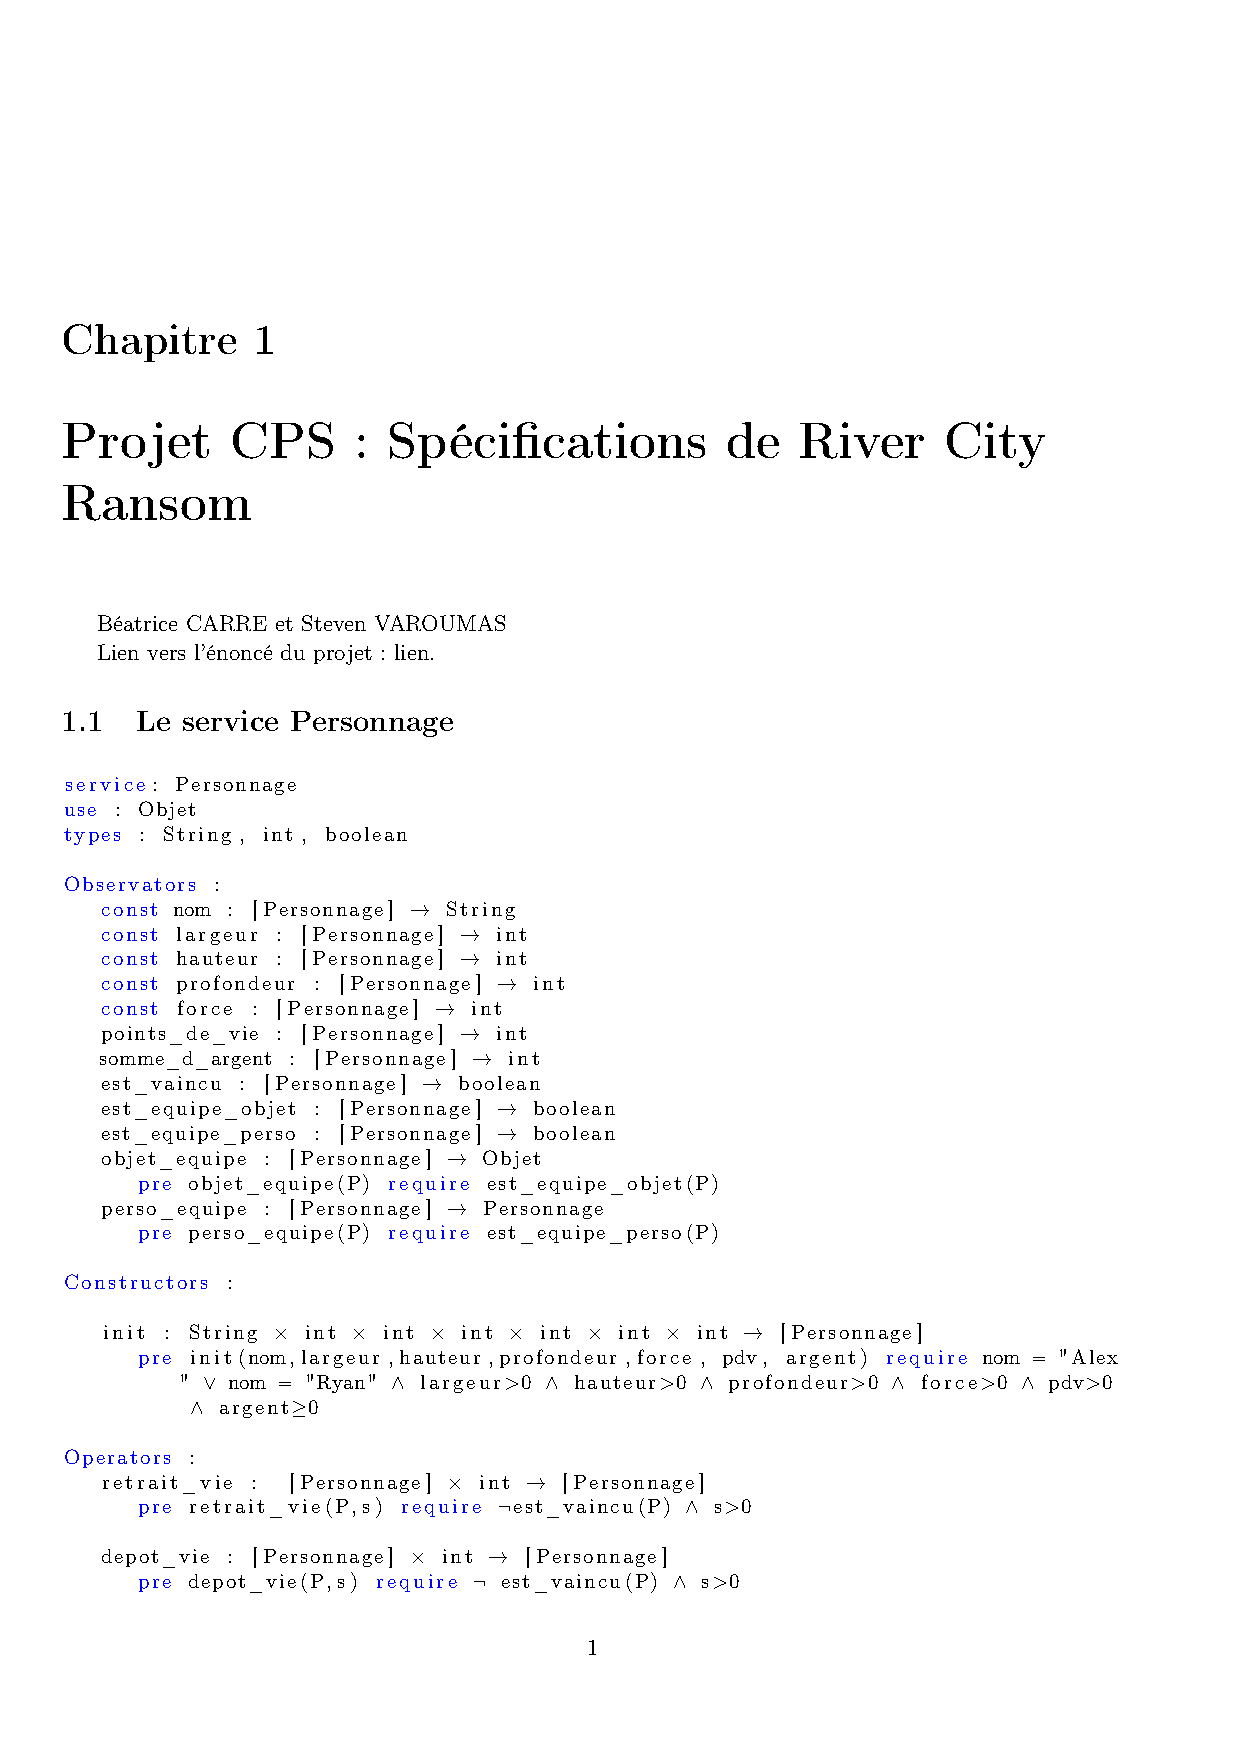
\includepdf[pages={-},pagecommand={},offset=2.cm 1cm]{../Spec/spec.pdf}

\newpage
\pagestyle{empty}
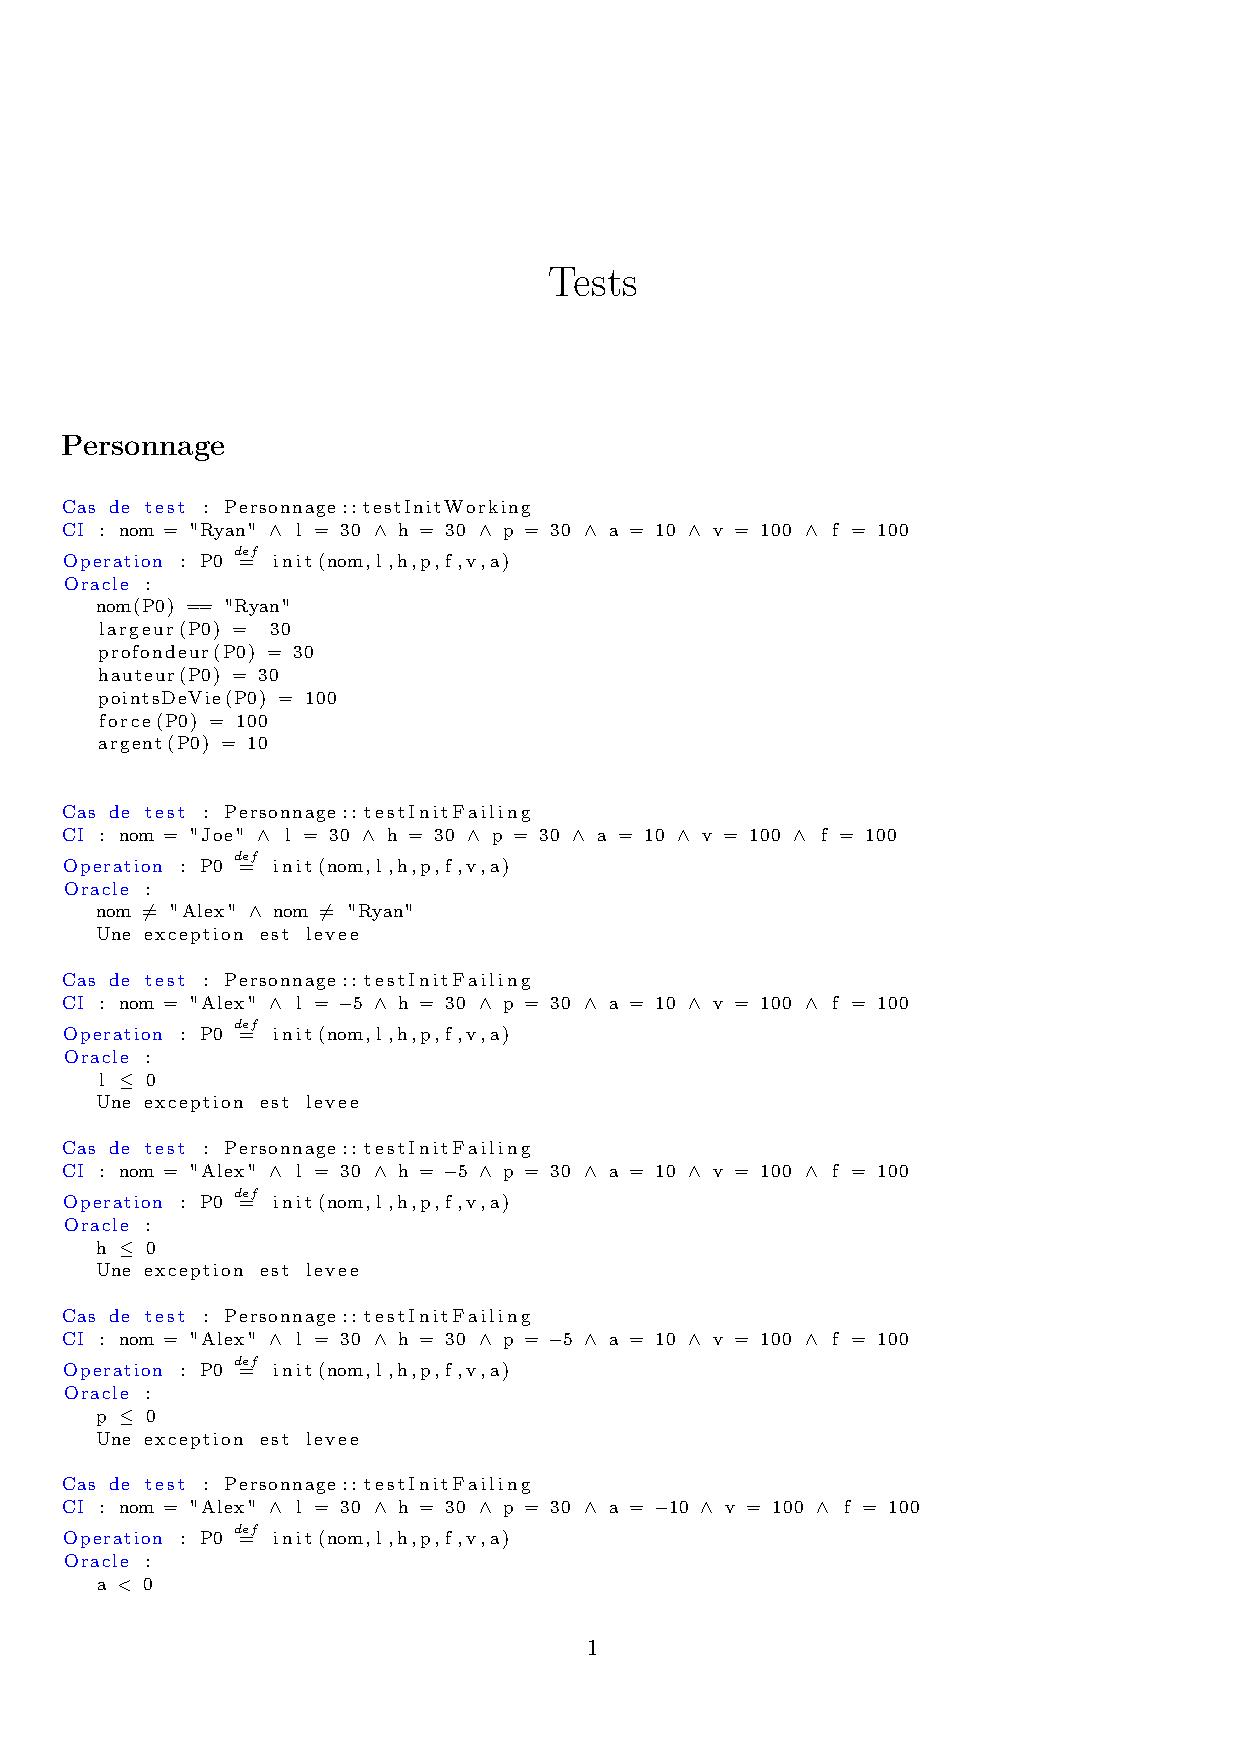
\includepdf[pages={-},pagecommand={},offset=2.cm 1cm]{../Tests/tests.pdf}
\end{document}
